\documentclass[10pt, twocolumn, letterpaper]{article}

% --- Packages ---
\usepackage[utf8]{inputenc}
\usepackage{geometry}
\geometry{margin=0.8in}
\usepackage{graphicx}
\usepackage{booktabs}
\usepackage{hyperref}
\usepackage{enumitem}
\setlist{nosep, leftmargin=1.2em}
% allow a full-width float to take most of a page top, and up to 2 top floats,
% so the results table does not get deferred to its own float page
\renewcommand{\dbltopfraction}{0.92}
\renewcommand{\dblfloatpagefraction}{0.5}
\renewcommand{\textfraction}{0.06}
\setcounter{dbltopnumber}{2}
\usepackage{titlesec}
\titlespacing*{\section}{0pt}{1.0ex plus .2ex}{0.5ex}
\titlespacing*{\subsection}{0pt}{0.6ex}{0.3ex}
\setlength{\textfloatsep}{6pt}
\setlength{\floatsep}{6pt}
\setlength{\intextsep}{6pt}
\setlength{\abovecaptionskip}{3pt}
\setlength{\belowcaptionskip}{1pt}
\setlength{\columnsep}{18pt}

% --- Document Information ---
\title{\vspace{-1ex}\large\textbf{Detecting Smart Money Concept Zones in Stock Candles with Deep Learning}\vspace{-1ex}}

\author{
    \small Nikola Baburov (\texttt{n.baburov@student.fontys.nl})
}

\date{\vspace{-2ex}}

\begin{document}

\maketitle

\begin{abstract}
Smart Money Concepts (SMC) are patterns that traders draw by hand on price charts to mark where the market may react; they are subjective, slow, and inconsistent between analysts. This project automates the most common one, the Fair Value Gap (FVG), directly from SPY stock-price data: it marks each candle, scores a confidence, and draws the zones as a chart overlay. It does not predict price; it finds and explains a known pattern. A five-model ladder (XGBoost, LSTM, CNN-LSTM, Transformer, xLSTM) is trained on a leakage-checked dataset with a strict time-ordered split. The headline finding is that the task is data-bound, not capacity-bound: a classic gradient-boosting model leads at macro-F1 0.738 (a 0-to-1 score of how well the rare zones are found, where 1.0 is perfect), the best neural detector reaches 0.713, and the neural models only catch up when given more data.
\end{abstract}

\section{Context}
This report summarises the SMC Data Challenge, an individual project for the AI-Advanced semester at Fontys, reviewed at peer and tutor checkpoints before this final delivery. The assignment asks for a Think-Big vision and a realistic MVP. The Think-Big vision is a full SMC assistant that detects the complete pattern vocabulary (Fair Value Gaps, break of structure, order blocks, liquidity sweeps) and explains its reasoning on any instrument. The MVP, delivered here, narrows that to one pattern on one symbol: a Fair Value Gap detector for SPY, a broad US stock-market fund.

A Fair Value Gap is a three-candle pattern that leaves a price range the market skipped over (Figure \ref{fig:main}, left); traders treat it as a zone where price may react later. The product is deliberately a detector with confidence scores and chart overlays, not a price forecaster, so a person can see which candles triggered each zone and how sure the model is.

\section{Data}
SPY one-minute bars are pulled from the Alpaca Markets API \cite{alpaca}; the free yfinance source was rejected after testing confirmed its hourly history is capped at 730 days, short of the 2016 start needed. Bars are filtered to the regular trading session (09:30 to 15:59 New York time) and resampled to one-hour candles anchored at the session open, avoiding pre-market contamination of the first bar.

Labels come from a custom rule, the \texttt{ValidFVGLabeller}: six criteria (five active at this scale) that mark a candle bullish-gap, bearish-gap, or neither, with the label set at the second bar after the pattern, the earliest point it is fully confirmed. A popular open-source library, \texttt{smartmoneyconcepts} \cite{smc}, was rejected after its gap routine was found to peek one bar into the future, a subtle leak that would inflate every score. Real gaps are rare (about 3 in 100 candles). To grow this minority, four liquid US index funds (SPY, QQQ, IWM, DIA) are pooled into one training set. The split is strictly by time and never shuffled, so the model is always tested on the future: train 2016 to 2021, tune 2022, test 2023 to 2025.

\section{Method}
Each example is a 60-by-5 window: the last sixty candles, each with five values (open, high, low, close, volume). Five models are compared on identical windows and the same untouched test set:
\begin{enumerate}
    \item \textbf{XGBoost}: the mandatory control, a gradient-boosted decision tree (many simple yes/no rules combined, each correcting the last) on hand-engineered features. With heavy window overlap the effective sample is small, where such models often beat neural networks.
    \item \textbf{LSTM} and \textbf{CNN-LSTM}: neural sequence models reading the raw candles in order; CNN-LSTM is the lead (carrier) architecture.
    \item \textbf{Transformer} and \textbf{xLSTM}: higher-capacity models, to test whether capacity, not data, is the missing ingredient.
\end{enumerate}
The five are listed in roughly ascending order of complexity; if the task simply needed more power the larger models would lead, and they do not. Because positives are rare, training uses weighted cross-entropy, which penalises missing a rare gap far more than missing a common non-gap. A lower-timeframe lever (resampling to 5-minute and 15-minute candles) plus automated hyperparameter search (Optuna) is applied to the carrier to test whether finer, more plentiful data lifts the neural models. XGBoost's lead is partly a fairer input (35 engineered features against raw prices), so the neural-to-neural ranking is the cleanest comparison.

\begin{figure*}[t]
\centering
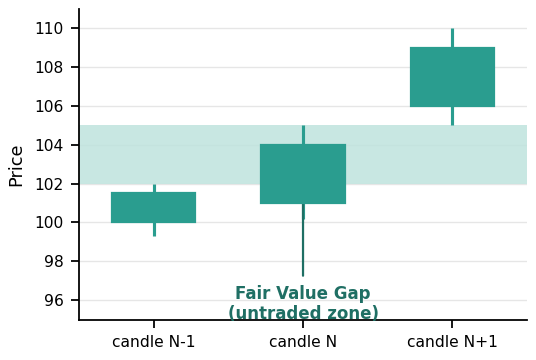
\includegraphics[width=0.37\textwidth]{fig_fvg.png}\hfill
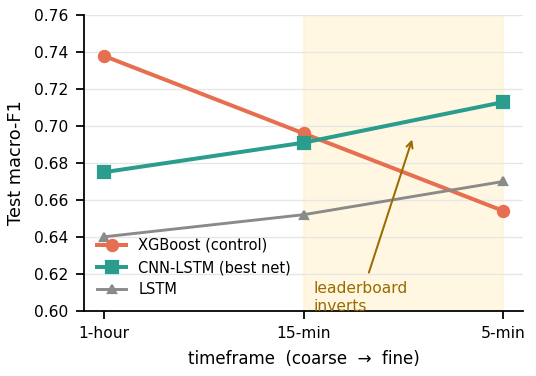
\includegraphics[width=0.37\textwidth]{fig_timeframe.png}
\caption{\textbf{Left:} a bullish Fair Value Gap: the shaded band is the price range the middle impulse candle skips. \textbf{Right:} the central result: as the timeframe gets finer (more training examples) the neural CNN-LSTM rises and overtakes the gradient-boosting control, whose hand-built hourly features weaken at finer scales. The bottleneck is data, not model size.}
\label{fig:main}
\end{figure*}

\begin{table}[t]
\centering
\footnotesize
\setlength{\tabcolsep}{4pt}
\begin{tabular}{@{}lll@{}}
\toprule
Model & Macro-F1 (95\% CI) & Best setup \\
\midrule
XGBoost \textit{(ctrl)} & \textbf{0.738} [.689,.779] & H1, pooled, eng. feats \\
CNN-LSTM & 0.713 [.708,.719] & 5m, pooled, tuned \\
LSTM & 0.640 [.604,.677] & H1, pooled \\
Transformer & 0.577 [.549,.602] & H1, pooled, unstable \\
xLSTM & 0.369 [.354,.384] & H1, SPY only \\
\bottomrule
\end{tabular}
\caption{Best result per model family on the unseen 2023 to 2025 test set. Pooled = SPY, QQQ, IWM, DIA. Macro-F1 averages equally over the three classes (no-gap, bullish, bearish gap); 1.0 is perfect, about 0.33 random. The 95\% range is a block bootstrap; overlapping ranges mean a tie.}
\label{tab:results}
\end{table}

\section{Results}
The primary metric is macro-F1 on the rare gap classes; accuracy is meaningless here, since always guessing "no gap" already scores 97 percent. Table \ref{tab:results} gives the best result per family.

Two findings stand out. First, on hourly data the XGBoost control leads every neural model. Second, the neural models climb when given more data: pooling four funds lifts them by 0.036 to 0.045, and a finer timeframe lifts them further until the CNN-LSTM overtakes XGBoost at 5-minute resolution (Figure \ref{fig:main}, right). The Transformer is the exception, held back by run-to-run instability rather than data. Together this is the project's central result: the task is data-bound, not capacity-bound, limited by how rarely clean gaps occur, not by model size.

A trade-simulation on the unseen years tests whether detections carry a real edge. Each detection becomes a bracket trade (a preset profit ceiling and a capped-loss floor) charged realistic costs (spread, slippage, a volatility-based minimum stop). Profit is measured in R, one unit of risk per trade: risk \$100 and +28R means \$2{,}800 over the three test years. After costs, only the two-to-one bracket on SPY stays positive at 15-minute resolution: a robust +58R for XGBoost and a marginal +28R (within run-to-run noise) for the tuned CNN-LSTM. The edge is absent on the other three funds.

\section{Validation}
A result is only as trustworthy as the protocol behind it:
\begin{itemize}
    \item \textbf{No peeking ahead}: an automatic test asserts every label uses only information available at the time, the check that caught the public library's leak.
    \item \textbf{Future-only testing}: the time-ordered split never lets a future candle inform a past prediction.
    \item \textbf{Honest uncertainty}: each headline number is a five-seed average with a confidence range, not one lucky run.
    \item \textbf{A floor and a human check}: majority-class and random baselines set the bar to beat, and a hand-annotated gold set sanity-checks predictions against expert judgement.
\end{itemize}
These ran as a ten-gate validation sprint; over 1{,}000 automated tests and saved checkpoints make every number reproducible.

\section{Product, Demo, and Future Work}
The deliverable is more than a notebook. An inspection tool writes an interactive chart shading each predicted zone by confidence, so detections can be audited candle by candle; a live harness paper-trades in real time through a risk-free practice account, with a multi-model fleet and deterministic replay. Because the task is data-bound, the next step is more data: more symbols and longer history. The detector extends to other SMC patterns (break of structure, order blocks) by adding labelling rules, not redesigning models; a longer live forward-test would show whether the thin 15-minute edge survives.

\section*{Acknowledgments}
Thanks to the Fontys AI-Advanced teaching staff for their guidance throughout the semester.

% --- References ---
\bibliographystyle{plain}
{\scriptsize \raggedright
\begin{thebibliography}{9}
\setlength{\itemsep}{0pt}\setlength{\parsep}{0pt}

\bibitem{alpaca}
Alpaca Markets. \textit{Market Data API}. https://alpaca.markets/

\bibitem{smc}
Attridge, J. \textit{smartmoneyconcepts} (open-source library). https://github.com/joshyattridge/smart-money-concepts

\end{thebibliography}
}

\end{document}
